% This file was created with tikzplotlib v0.10.1.
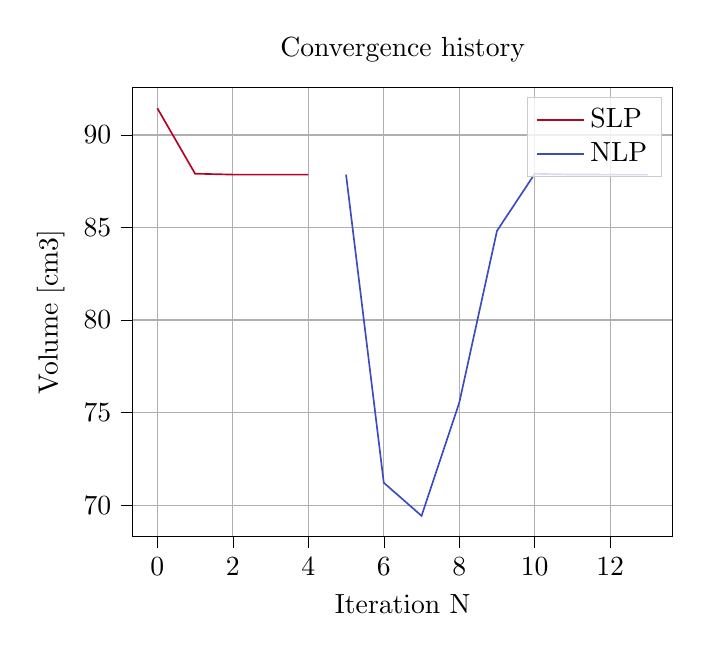
\begin{tikzpicture}

\definecolor{darkgray176}{RGB}{176,176,176}
\definecolor{firebrick180438}{RGB}{180,4,38}
\definecolor{lightgray204}{RGB}{204,204,204}
\definecolor{royalblue5976192}{RGB}{59,76,192}

\begin{axis}[
legend cell align={left},
legend style={fill opacity=0.8, draw opacity=1, text opacity=1, draw=lightgray204},
tick align=outside,
tick pos=left,
title={Convergence history},
x grid style={darkgray176},
xlabel={Iteration N},
xmajorgrids,
xmin=-0.65, xmax=13.65,
xtick style={color=black},
y grid style={darkgray176},
ylabel={Volume [cm3]},
ymajorgrids,
ymin=68.3204538738177, ymax=92.5436111134765,
ytick style={color=black}
]
\addplot [semithick, firebrick180438]
table {%
0 91.4425585116738
1 87.9070802673692
2 87.8579447685309
3 87.8579100270034
4 87.8579100269807
};
\addlegendentry{SLP}
\addplot [semithick, royalblue5976192]
table {%
5 87.8579100265101
6 71.2089614235501
7 69.4215064756204
8 75.530995159555
9 84.8208410946121
10 87.9000340028275
11 87.8608683972871
12 87.8579431308577
13 87.8579102591606
};
\addlegendentry{NLP}
\end{axis}

\end{tikzpicture}
